\documentclass[a4paper]{article}

%%%%%%%%%%%%%%%%%%%%%%%%%%%%%%%%

\usepackage[utf8]{inputenc}
\usepackage[T1]{fontenc}
\usepackage[francais]{babel}

\usepackage{graphicx}
\usepackage{wrapfig}
\usepackage{algorithm2e}
\usepackage{amssymb}
\usepackage{amsthm}
\usepackage{amsmath}
\usepackage{amsfonts}
\usepackage{enumitem}
\usepackage{stmaryrd}
\setlength{\textwidth}{370pt}

\usepackage{titling}
%%%%%%%%%%%%%%%%%%%%%%%%%%%%%%%%


\newtheorem{definition}{Définition}
\newtheorem{ex}{Exemple}
\newtheorem{prop}{Proposition}
\newtheorem{theorem}{Théorème}
\newtheorem{dem}[theorem]{Démonstration}
\newtheorem{propriete1}{Propriété}[section]
\newtheorem{loi}{Loi de Composition}
\newtheorem{lem}{Lemme}
\newtheorem{slem}{SubLemma}
\newcommand{\overbar}[1]{\mkern 1.5m \overline{\mkern-1.5mu#1\mkern-1.5mu}\mkern 1.5mu}
\renewcommand\thesection{\Roman{section}}

%%%%%%%%%%%%%%%%%%%%%%%%%%%%%%%%

\title{Les points rationnels des courbes elliptiques}
\author{Théophile Hontang}
\date{\today}

\begin{document}
\maketitle
\tableofcontents
\newpage
\section*{Introduction}

\newpage


\section{Géométrie et Arithmétique}
\subsection{Groupe des Rationnels}
\begin{figure}[h]
\centering
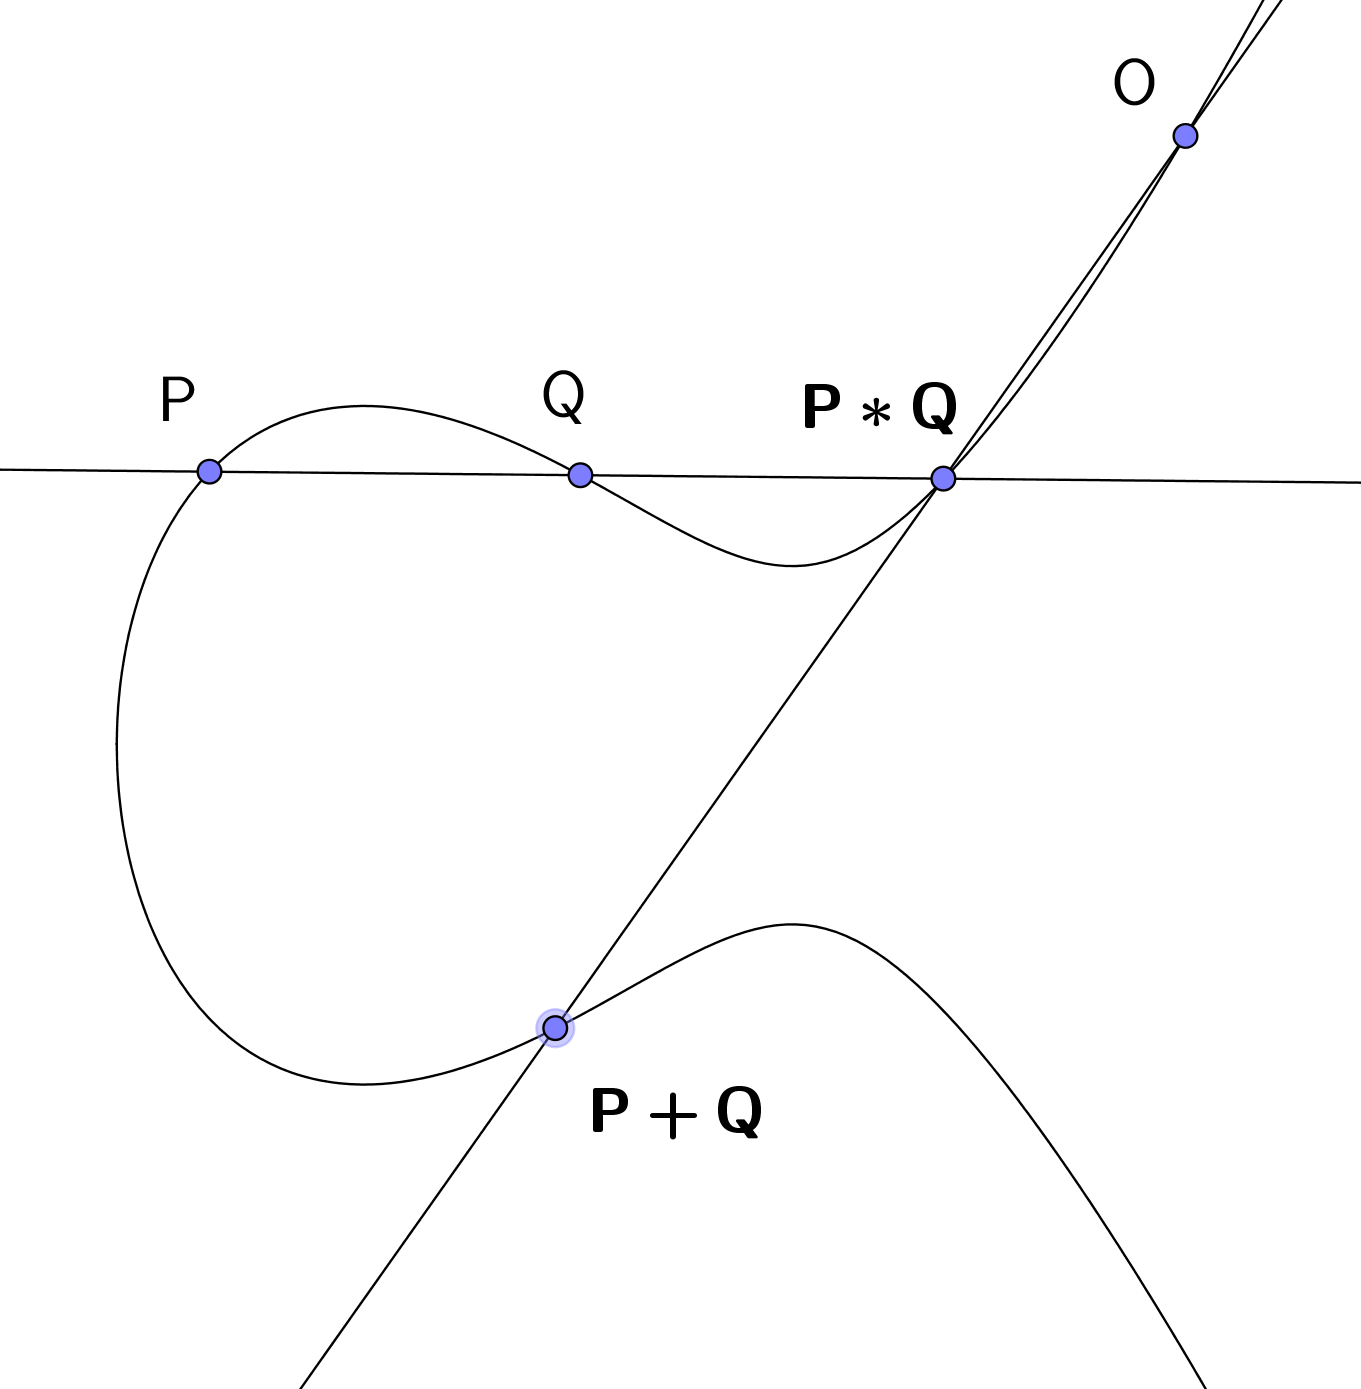
\includegraphics[scale=0.2]{addition.png}
\caption{Loi d'addition}
\label{neutre}
\end{figure} 
On note $I(C_{1} \cap C_{2},P)$ la multiplicité de $P$, point d'intersection de $C_{1} \cap C_{2}$
\begin{theorem}[Bézout]
Soit $C_{1}$ et $C_{2}$ deux courbes projectives avec des composantes non communes. Alors :
\begin{equation*}
\sum\limits_{P \in C_{1} \cap C_{2}} I(C_{1} \cap C_{2},P)=(\deg  C_{1})(\deg C_{2})
\end{equation*}
\end{theorem}
Soit $C$ une courbe elliptique. Elle est donnée par une équation de la forme \\ $F(X,Y,Z)=0$ où F est un polynôme homogène de degré 3. Nous verrons dans la prochaine section qu'une réduction est possible (dite de Weierstrass). \\
Soit $L \in \mathbb{P}^2$ une droite. Par le théorème de Bézout, $L$ intersecte $C$ en trois points(Ces points ne sont pas forcément distincts).\\
Définissons la loi de composition $+$ de $C$ par la règle suivante.

\begin{loi}
Soient $P,Q \in C$, $L$ la droite joignant $P$ et $Q$ (ou la tangente si $P=Q$), et $P*Q$ le troisième point d'intersection  de $L$ par $C$.
Soit $L'$ la droite joignant $P*Q$ et $O$. Alors $P+Q$ est le point tel que $L'$ intersecte $C$ aux points $P*Q$, $O$ et $P+Q$. C'est à dire:
\begin{equation*}
P+Q=O*(P*Q)
\end{equation*}
\end{loi}

\begin{prop}
$C$, muni de la loi de composition $+$, est un groupe abélien avec $O$ comme élément neutre.
E vérifie alors les propriétés suivantes :
\begin{enumerate}
\item Si $L$ intersecte $C$ aux points $P,Q$ et $R$ alors
\begin{equation*}
(P+Q)+R=O
\end{equation*}
\item $\forall P \in C$, 
\begin{equation*}
P+O=P
\end{equation*}
\item $\forall P,Q \in C$
\begin{equation*}
P+Q=Q+P
\end{equation*}
\item Soit $P \in C$.Il existe un point, qu'on note $-P$, tel que
\begin{equation*}
P+(-P)=O
\end{equation*}
\item Soit $P,Q,R \in C$. Alors
\begin{equation*}
(P+Q)+R=P+(Q+R)
\end{equation*}
\end{enumerate}
\end{prop}
\begin{proof} 
\begin{enumerate}
\item Trivial par la loi de composition. 
\item (\it{Voir Figure 2}) $L$ et $L'$ coïncident. $L$ intersecte $C$ aux points $P,O,R$ et $L'$ intersecte $C$ aux points $P+O,O,R$ d'où $P+O=P$. 
\item Par construction.
\item (\it{Voir Figure 2}) La droite, qui passe par $P$ et $O$, intersecte $C$ au point qu'on nomme $R$. En utilisant 1) et 2), nous obtenons 
\begin{equation*}
O=(P+O)+R=P+R
\end{equation*}
\item (\it{Voir Figure 3})
\end{enumerate}

\begin{figure}[h]
\centering
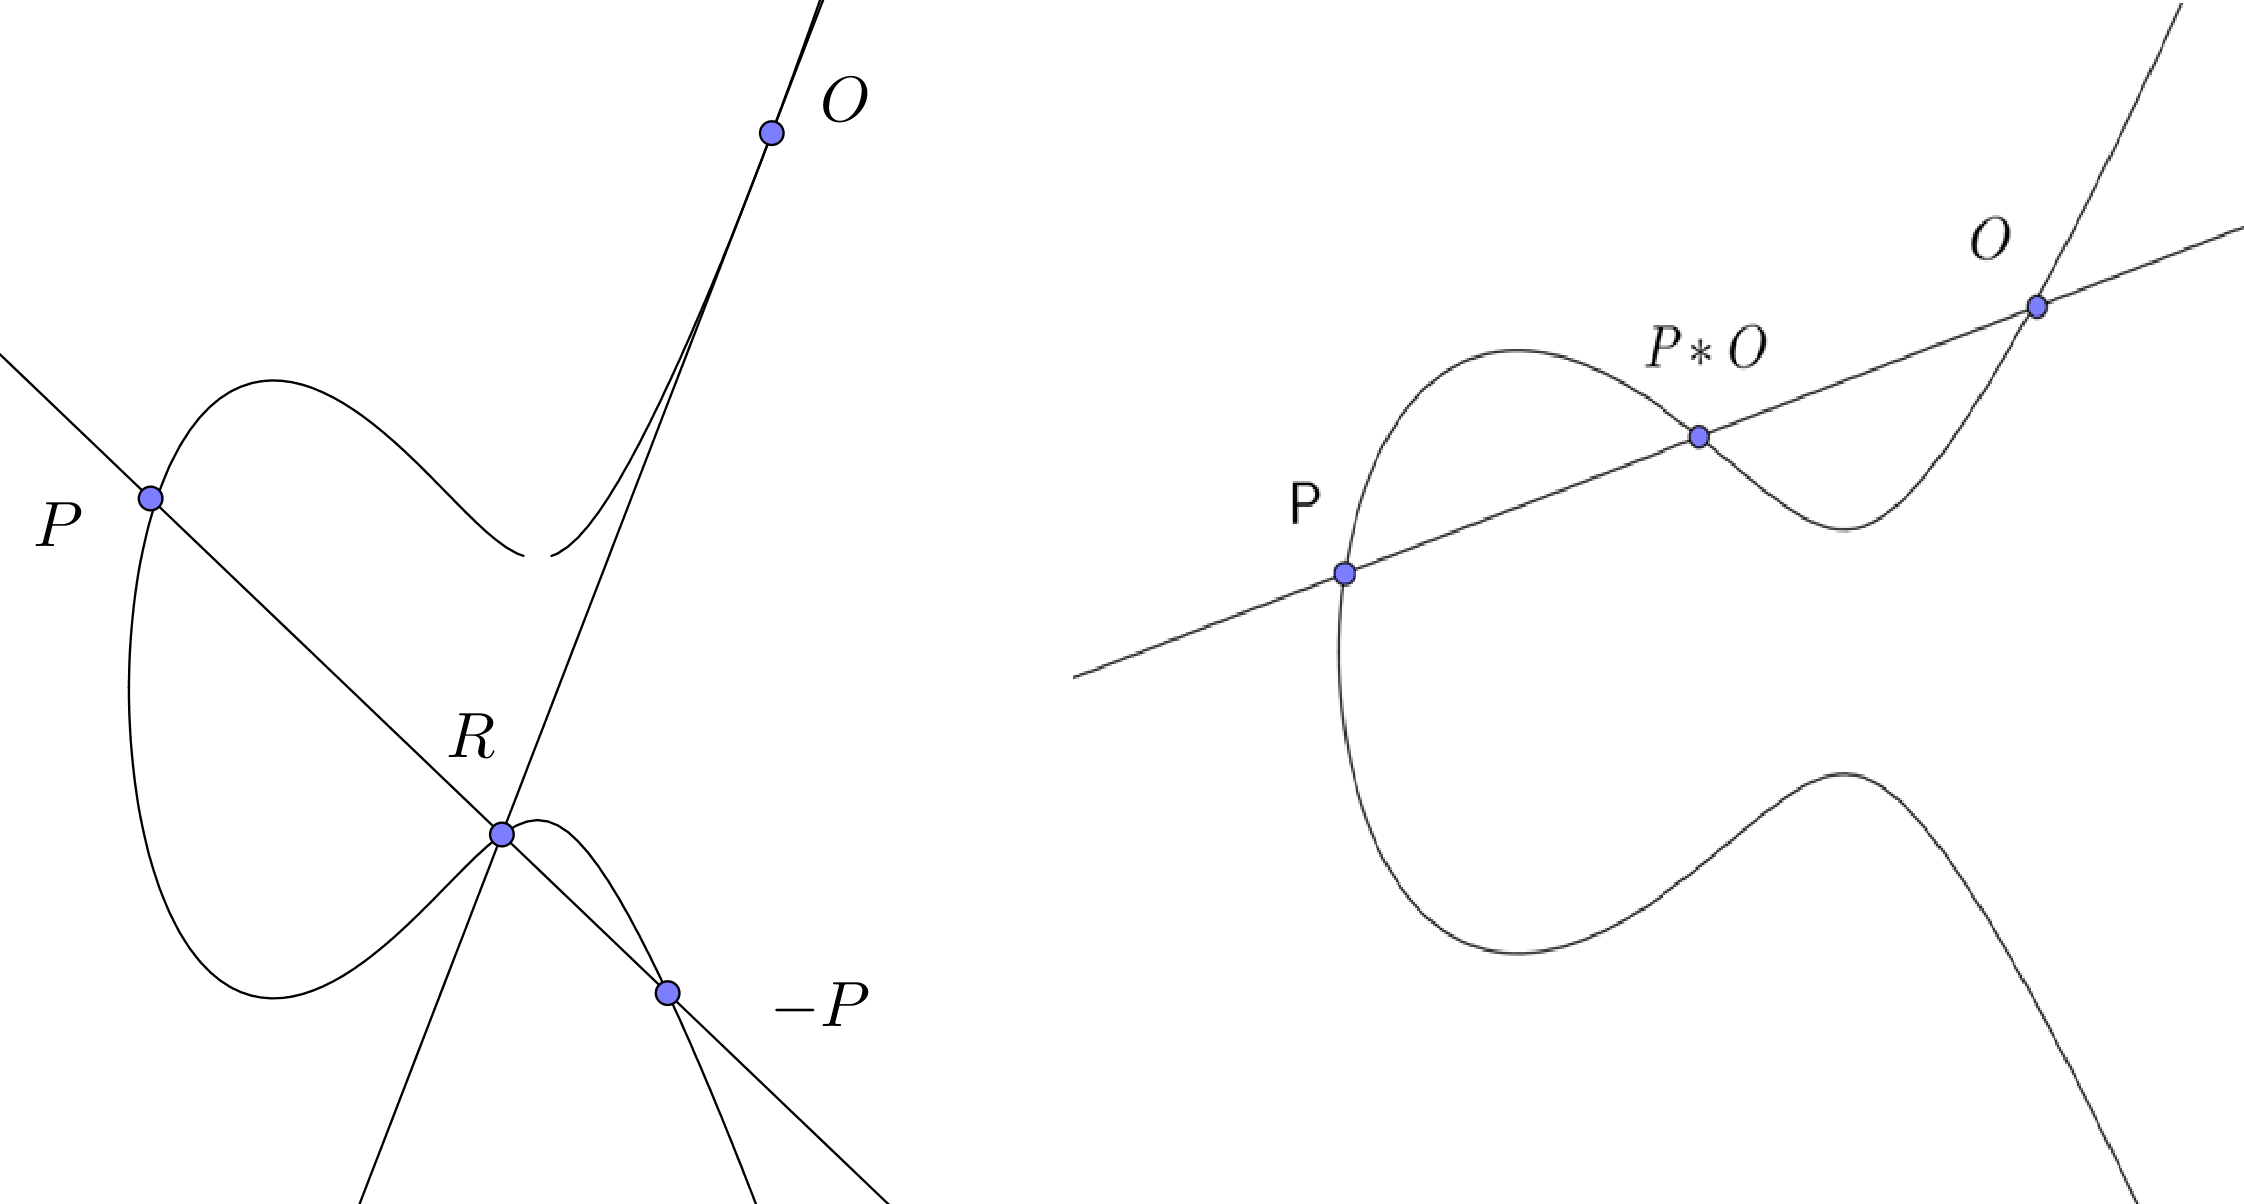
\includegraphics[scale=0.10]{ensemble.png}
\caption{Opposé et Élément neutre}
\label{neutre}
\end{figure}
\begin{figure}[h]
\centering
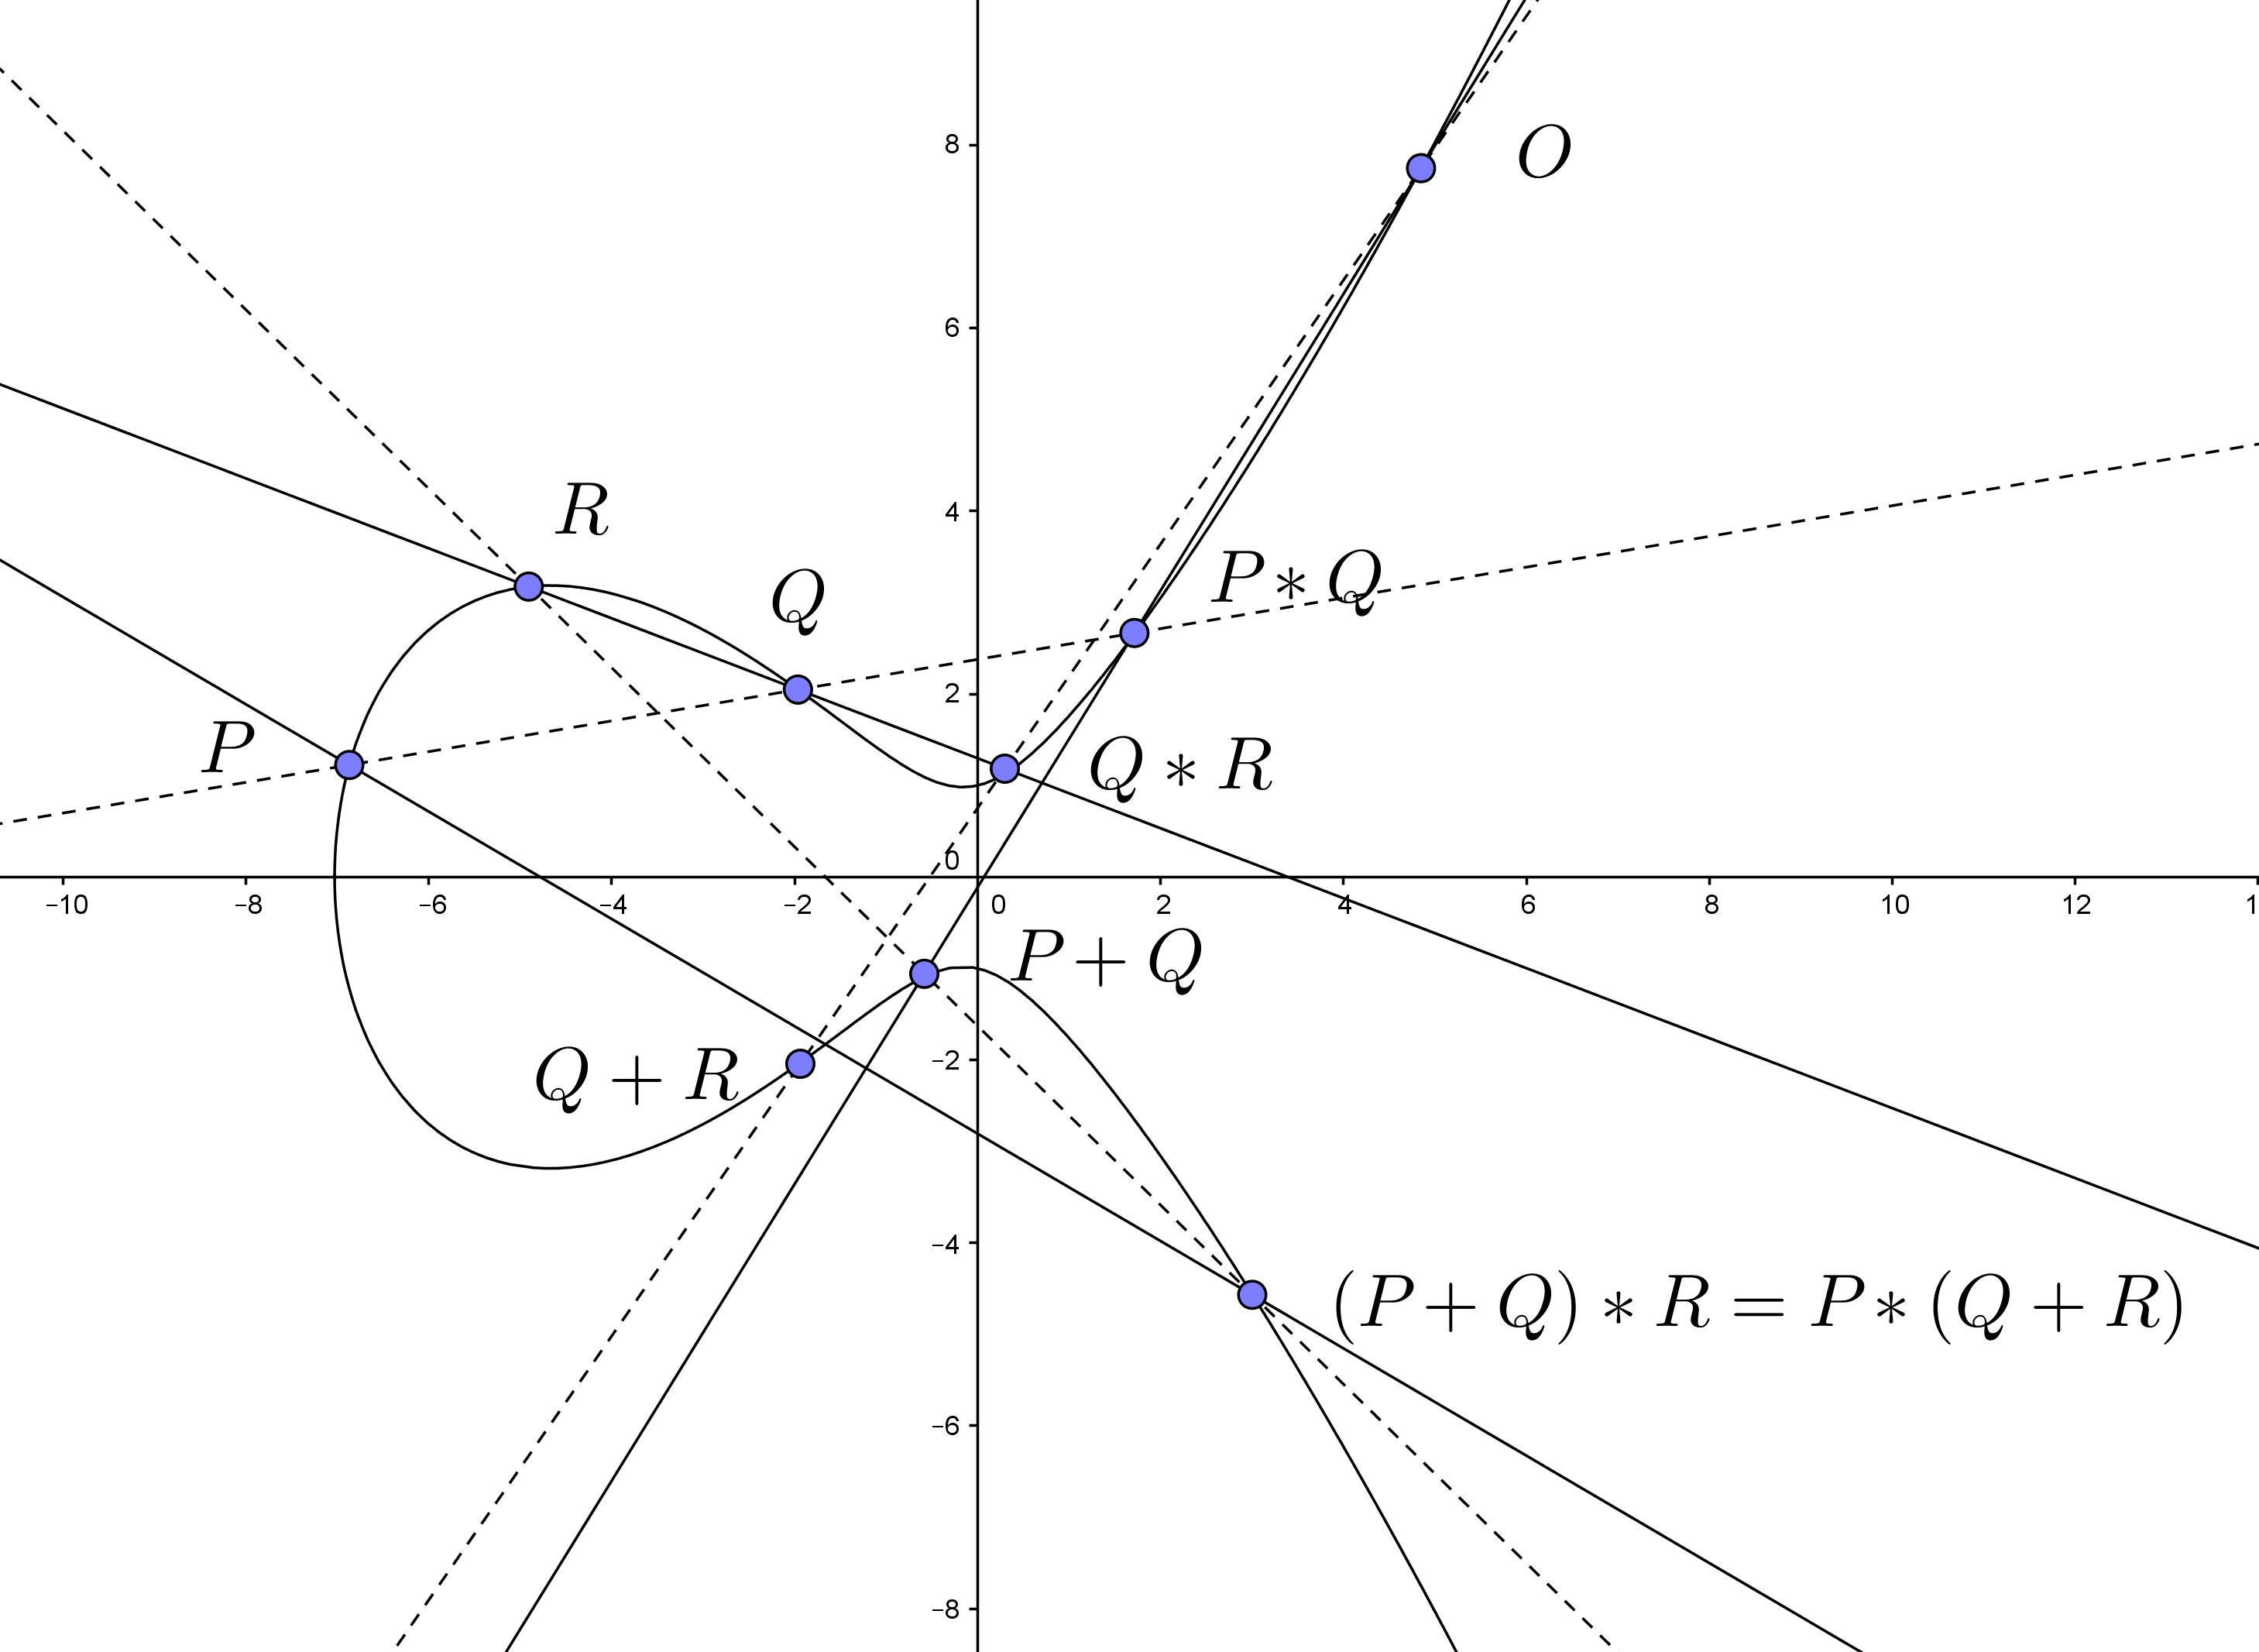
\includegraphics[scale=0.08]{associativite.png}
\caption{Associativité}
\label{neutre}
\end{figure}

\end{proof}

\newpage
\subsection{Weierstrass et formule de duplication}

Une courbe elliptique $C$ est donnée par $F(x,y)=0$ où $\deg_{x}F=\deg_{y}F=3$.
Nous nous plaçons dans le plan projectif $\mathbb{P}^2$. L'idée est de réaliser une transformation projective pour réduire la forme de $F$. Pour cela, prenons un point rationnel $\mathcal{O}$ sur $C$. Soit $Z=0$ la tangente de $C$ en $\mathcal{O}$. Cette droite coupe $C$ en un autre point qu'on nomme $P$. Soit $X=0$  la tangente de $C$ en $P$, elle coupe $C$ en un point $Q$.
On choisit $Y=0$ une droite qui passe par $\mathcal{O}$ mais différent de $Z=0$. En posant $x=X/Z$ et $y=Y/Z$, on obtient une transformation projective et l'équation est alors de la forme dite de Weierstrass :
\begin{equation*}
F: y^2=ax^3+bx^2+cx+d
\end{equation*}
Le lecteur pourra se reporter sur le livre \cite{ref2} pour les calculs. \\
La loi du groupe sur la forme de Weierstrass reste identique à celle vue précédemment. Dans ce cas , l'élément neutre $\mathcal{O}$ est un point à l'infini. Le point $P*Q=(x,y)$, défini comme précédemment, donne le point $P+Q=(x,-y)$, point symétrique par rapport à un axe.
Nous remarquons alors que si $P=(x,y) \in C$ alors $-P=(x,-y) \in C$.

\begin{prop}[Formule de Duplication] 
 Soit $C$ une courbe elliptique de la forme de Weierstrass $(C): y^2=x^3+ax^2+bx+c$.
\begin{enumerate}
\item Soient $P_{i}=(x_{i},y_{i}) \in C$ pour $i \in \{1,2\}$.
alors $P_{1}+P_{2}=(x_{3},y_{3})$ avec 
\begin{equation*}
x_{3}=\lambda^2-a-x_{1}-x_{2} \hspace{1cm} y_{3}=\lambda x_{3}+\nu
\hspace{1cm}
\lambda=\frac{y_{2}-y_{1}}{x_{2}-x_{1}}
\end{equation*}
\item Soit $P_{0}=(x_{0},y_{0}) \in C$. Alors la coordonnée en $x$ de $2P$ est :
\begin{equation*}
x(2P)=\frac{x_{0}^4-2bx_{0}^2-8cx_{0}+b^2-4ac}{4x_{0}^3+4ax_{0}^2+4bx_{0}+4c}
\end{equation*}
\end{enumerate}
\end{prop}

\begin{proof}
1) Soient $P_{1}*P_{2}=(x_{*},y_{*})$.
La droite joignant $P_{1}$ et $P_{2}$ est définie par l'équation $y=\lambda x+\nu$ avec $\lambda=\frac{y_{2}-y_{1}}{x_{2}-x_{1}}$ et $\nu=y_{1}-\lambda x_{1}$.
L'intersection de cette droite avec $C$ est définie par :
\begin{equation*}
x^3+(a-\lambda^2)x^2+(b-2\lambda\nu)x+(c-\nu^2)=0
\end{equation*}
Les trois racines de ce polynôme sont $x_{1},x_{2}$ et $x_{*}$.
Par les relations de Viète qui expriment les coefficients du polynôme par les racines, nous obtenons :
\begin{equation*}
a-\lambda^2=-(x_{1}+x_{2}+x_{3})
\end{equation*}
Comme $x_{3}=x_{*}$ et $y_{3}=-y_{*}$, nous obtenons bien les coordonnées de $P_{1}+P_{2}$. \\
2) $P*P$ est obtenu par l'intersection de $C$ et de la tangente de $C$ en $P$. La pente est $\lambda={\frac{dy}{dx}}(P_{0})=\frac{f'(x_{0})}{2y_{0}}$. En substituant $\lambda$ dans les équations obtenues en 1) et en remplaçant $y^2$ par $x^3+ax^2+bx+c$, nous obtenons le résultat.

\end{proof}

\newpage
\subsection{Poins d'ordre fini} 
\begin{definition}
Un point $P$ est d'ordre fini $m$ si 
\begin{equation*}
mP= \underbrace{P+...+P}_{m fois} = \mathcal{O}
\end{equation*} 
Sinon P est d'ordre infini.
\end{definition}

\begin{definition}
Soit $C$ une courbe cubique donnée par 
\begin{equation*}
C:y^2=f(x)=x^3+ax^2+bx+c
\label{neutre}
\end{equation*} 
est dite $\mathbf{non-singuliere}$ si $f$ et $f'$ ont aucune racine commune; i.e f n'admet que des racines simples.
\end{definition}

\begin{theorem}[Points d'ordre $2$ et $3$]
Soit $C$ une courbe cubique non-singulière donnée par \eqref{neutre}
\begin{enumerate}
\item Un point $P=(x,y)$ sur $C$ est d'ordre 2 ssi $y=0$.
\item $C$ a quatre points d'ordre divisant 2.
Ces quatre points forment un groupe isomorphe à $\mathbb{Z}/2\mathbb{Z} \times \mathbb{Z}/2\mathbb{Z}$
\item Un point $P=(x,y)$ est d'ordre 3 ssi x est racine du polynôme :
\begin{equation*}
\chi(x)= 3x^4+4ax^3+6bx^2+12cx+4ac-b^2
\end{equation*}
\item C a neuf points d'ordre divisant 3. Ces neuf points  forment un groupe isomorphe à 
$\mathbb{Z}/3\mathbb{Z} \times \mathbb{Z}/3\mathbb{Z}$.
\end{enumerate}
\end{theorem}
\begin{proof}

\end{proof}


\begin{theorem}[Nagell-Lutz \cite{ref3}
\cite{ref4}]
Soit 
\begin{equation*}
y^2=x^3+ax^2+bx+c
\end{equation*}
une courbe cubique non-singulière avec $a,b,c \in \mathbb{N}$ et D le discriminant; i.e
\begin{equation*}
D=-4a^3c+a^2b^2+18abc-4b^3-27c^3
\end{equation*}
Soit $P=(x,y)$ un point rationnel d'ordre fini. \\
Alors $x,y \in \mathbb{N}$ et soit P est d'ordre 2, soit y divise D.
\end{theorem}

\begin{theorem}[\cite{ref6} \cite{ref7}]
Soit $C$ une courbe cubique rationnel non-singulière, et supposons que $C(\mathbb{Q})$ contient un point d'ordre fini $m$. Alors
\begin{equation*}
1 \leqslant m \leqslant 10 \; \; \; ou \; \; \; m=12
\end{equation*}
\end{theorem}
Dans la prochaine section, nous allons montrer que $C(\mathbb{Q})$ est de type fini, i.e $C(\mathbb{Q}) \simeq \mathbb{Z}^r \times C(\mathbb{Q})_{tors}$ où $r$ est le rang de la courbe. Le sous-groupe de torsion $C(\mathbb{Q})_{tors}$ peut alors être identifié à quinze groupes :
\begin{equation*}
\mathbb{Z}/n\mathbb{Z} \hspace{0.5cm} 0 \leqslant n \leqslant 10 \hspace{0.3cm} ou\hspace{0.3cm} n=12
\end{equation*}
\begin{equation*}
\mathbb{Z}/2\mathbb{Z} \times \mathbb{Z}/2n\mathbb{Z} \hspace{0.5cm}  1\leqslant n \leqslant 4
\end{equation*}


\newpage
\section{Théorème de Mordell-Weil}
\begin{theorem}[\cite{ref5}]
Soit $C$ une courbe elliptique définie par l'équation
\begin{equation*}
C : y^2=x^3+ax^2+bx
\end{equation*}
avec $a,b \in \mathbb{N}$. Alors $C(\mathbb{Q})$ est un groupe abélien de type fini.
\end{theorem}


\begin{proof}

\begin{theorem}[Descente]
Soit $\Gamma$ un groupe commutatif et soit la fonction
\begin{equation*}
h : \Gamma \rightarrow [0, \infty]
\end{equation*}
vérifiant les propriétés suivantes : 
\begin{enumerate}
\item Quelque soit $M$ réel, $\{P \in \Gamma : h(P) \leqslant M\}$ est fini
\item Quelque soit $P_{0}$ point de $\Gamma$, il existe $\kappa_{0}$ tel que 
\begin{equation*}
h(P+P_{0}) \leqslant 2h(P) + \kappa_{0} \; \; \; \; \forall P \in \Gamma   
\end{equation*}
\item Il existe une constante $\kappa$ telle que :
\begin{equation*}
h(2P) \geqslant 4h(P) - \kappa \; \; \; \; \forall P \in \Gamma 
\end{equation*}
\item  $|\Gamma:2\Gamma|$ est fini
\end{enumerate}
Alors $\Gamma$ est de type fini
\end{theorem}

\begin{proof}
D'après 4), il existe un nombre fini de représentants de classe de $\Gamma / 2\Gamma$ qu'on note $Q_{1},Q_{2},...,Q_{n}$. Cela signifie que pour tout $P \in \Gamma$, il existe un indice $i_{1}$, dépendant de $P$, tel que $P-Q_{i_{1}} \in 2\Gamma$. On peut alors noter $P-Q_{i_{1}}=2P_{1}$ pour $P_{1} \in \Gamma$. En procédant de même, on peut écrire :
\begin{align*}
P-Q_{i_{1}}&=2P_{1} \\
P_{1}-Q_{i_{2}}&=2P_{2} \\
P_{2}-Q_{i_{3}}&=2P_{3} \\
\vdots \\
P_{m-1}-Q_{i_{m}}&=2P_{m}
\end{align*}
où $Q_{i_{1}},...,Q_{i_{m}}$ sont choisis parmi les représentants $Q_{1},...,Q_{n}$ et $P_{1},...,P_{m} \in \Gamma$.
En substituant la j-ème ligne dans la(j-1)-ème ligne, et par une rapide récurrence, nous obtenons :
\begin{equation}
P=Q_{i_{1}}+2Q_{i_{2}}+...+2^{m-1}Q_{i_{m}}+2^mP_{m}
\end{equation}
Nous allons appliquer la méthode de descente infinie dans le but de contrôler $P_{m}$ par la hauteur.
Par 2), $h(P-Q_{i}) \leqslant 2h(P) + \kappa_{i} \leqslant 2h(P) + \kappa'$ pour tout $P \in \Gamma $ et $\kappa' =\displaystyle \max_{1 \leqslant j \leqslant n} k_{j}$. Par 3), pour tout $j \in  \llbracket 1,n \rrbracket$
\begin{equation*}
4h(P_{j}) \leqslant h(2P_{j})+\kappa=h(P_{j-1}-Q_{i_{j}})+\kappa \leqslant
2h(P_{j-1})+\kappa'+\kappa
\end{equation*}
\begin{equation*}
h(P_{j}) \leqslant \frac{3}{4}h(P_{j-1})-\frac{1}{4}(h(P_{j-1})-(\kappa'+\kappa))
\end{equation*}
Si $(*) h(P_{j-1})\geqslant \kappa'+\kappa$ alors $h(P_{j}) \leqslant \frac{3}{4}h(P_{j-1})$. Tant que la condition $(*)$ est vraie, le prochain point dans la suite $P_{1},...,P_{n}$ possède une hauteur plus petite. Il existe un indice $m$ tel que $h(P_{m}) \leqslant \kappa'+\kappa$.
Ainsi, l'ensemble
\begin{equation*}
\{Q_{1},Q_{2},...,Q_{n}\} \cup \{P \in \Gamma ; h(P) \leqslant \kappa'+\kappa\}
\end{equation*}
engendre $\Gamma$. Par 1) et 4), l'ensemble est fini d'où $\Gamma$ est de type fini.
\end{proof}

\begin{definition}
Soit $t \in \mathbb{Q}$ et $t=p/q$ avec $pgcd(p,q)=1$. \\
La \textbf{hauteur} $H(t)$ de $t$ est défini par 
\begin{equation*}
H(t)=max\{| p |,| q |\}
\end{equation*}
\end{definition}

\begin{definition}
La \textbf{hauteur} sur $C(\mathbb{Q})$ est la fonction : 
\begin{equation*}
h : C(\mathbb{Q}) \rightarrow \mathbb{R} 
\end{equation*}
\begin{equation*}
h(P(x,y))=log(H(x))
\end{equation*}
\end{definition} 
La hauteur fera office de fonction et $C(\mathbb{Q})$ de groupe commutatif dans le théorème de la descente.
Les quatre hypothèses sur $h$ sont démontrés ci-dessous et ainsi le théorème de Mordell sera démontré.

\begin{lem}
L'ensemble des rationnels, dont la hauteur est plus petit qu'un nombre fixé, est un ensemble fini. \\
$\forall M \in \mathbb{R}, \{P \in \Gamma : h(P) \leqslant M\}$ est fini
\end{lem}

\begin{proof}
Si $x=\frac{m}{n}$ est plus petite qu'une constante, alors $\mid m \mid$ et $\mid n \mid$ sont plus petites que cette constante donc il existe un nombre fini de possibilités pour $m$ et $n$.
\end{proof}

\begin{lem}
$\forall P_{0} \in \Gamma$, il existe $\kappa_{0}$ (dépendant de $P_{0},a,b,c$) tel que 
\begin{equation}
h(P+P_{0}) \leqslant 2h(P) + \kappa_{0} \; \; \; \; \forall P \in \Gamma   
\end{equation}
\end{lem}


\begin{proof}
Par des opérations élémentaires, on peut montrer que chaque point rationnel $P=(x,y)$ peut être mis sous la forme suivante :
\begin{equation} \label{neutr}
x=\frac{m}{e^2} \hspace{1cm} y=\frac{n}{e^3} \hspace{1cm} e,m,n \in \mathbb{N^*} 
\end{equation}
avec $pgcd(e,m)=1$ et $pgcd(e,n)=1$. \\
En la mettant dans l'équation de la cubique, on a :
\begin{equation*}
n^2=m^3+ae^2m^2+be^4m+ce^6
\end{equation*}
En utilisant le fait que :
$\mid m \mid \leqslant H(P)$ et $e^2 \leqslant H(P)$
et par l'inégalité triangulaire, on a :
\begin{equation}
| n^2 | \leqslant K H(P)^3   \hspace{1cm} K=\sqrt{1+|a|+|b|+|c|}.
\end{equation}
Supposons que $P=(x,y) \notin \{P_{0},-P_{0},\mathcal{O} \}$ avec $ P_{0}=(x_{0},y_{0})$ et que $P+P_{0}=(\xi,\eta)$.
La formule de duplication nous donne :
\begin{align*}
\xi+x+x_{0}&=\Big(\frac{y-y_{0}}{x-x_{0}}\Big)^2-a \\
\iff \xi&= \frac{Ane+Bm^2+Cme^2+De^4}{Em^2+Fme^2+Ge^4} \hspace{1cm}       \\ 
\end{align*}
avec $A,B,C,D,E,F,G \in \mathbb{N}$.  
D'où $H(\xi) \leqslant max\{| Ane+Bm^2+Cme^2+De^4 |, | Em^2+Fme^2+Ge^4 | \}$
Par les inégalités obtenues en  et , 
\begin{equation*}
H(P+P_{0})=H(\xi)\leqslant max \{| AK | + | B | + | C |+| D |, | E | + | F | + | G |\}H(P)^2
\end{equation*}
En appliquant la fonction logarithme, on a bien le résultat avec
$
\kappa_{0}=log(max \{| AK | + | B | + | C |+| D |, | E | + | F | + | G |\})$
\end{proof}

\begin{lem}
Il existe une constante $\kappa$(dépendant de $a,b,c$) tel que :
\begin{equation}
h(2P) \geqslant 4h(P) - \kappa \; \; \; \; \forall P \in \Gamma 
\end{equation}
\end{lem}
\begin{proof}
Soit $P=(x,y)$ un point qui n'est pas d'ordre 2 et $2P=(\xi,\eta)$.
\textit{Formule de duplication}
\begin{equation*}
\xi +2x=\Big( \frac{f'(x)}{2y}\Big)^2-a
\end{equation*}
\begin{equation*}
\xi=\frac{f'(x)^2-(8x+4a)f(x)}{4f(x)}=\frac{x^4+...}{4x^3+...}
\end{equation*}
$\xi$ est le quotient de deux polynômes qui n'ont aucune racine complexe commune car $C$ est non-singulière. \\
Comme $h(P)=h(x)$ et $h(2P)=h(\xi)$, nous allons prouver 
\begin{equation*}
h(\xi) \leqslant 4h(x)-\kappa
\end{equation*}


\begin{slem}
Soit $\phi$ et $\psi$ des polynômes à coefficients entiers et aucune racine complexe commune. Soit $d=max(deg(\phi),deg(\psi))$
\begin{enumerate}[label=\roman*)]
\item Il existe un entier $R \geqslant 1$ dépendant de $\phi$ et $\psi$ telle que, pour tout rationnel $m/n$,
\begin{equation*}
pgcd\Big(n^d\phi\Big(\frac{m}{n}\Big),n^d\psi\Big(\frac{m}{n}\Big)\Big) \mid R
\end{equation*}
\item Ils existent des constantes $\kappa_{1}$ et $\kappa_{2}$ (dépendant de $\phi$ et $\psi$) telle que, pour tout rationnel $m/n$,
\begin{equation*}
dh\Big(\frac{m}{n}\Big)-\kappa_{1} \leqslant h\Big(\frac{\phi(m/n)}{\psi(m/n)}\Big) 
\end{equation*}
\end{enumerate}
\end{slem}
\begin{proof}
Posons $deg(\phi)=d$ et $deg(\psi)=e\leqslant d$. On peut écrire
\begin{align*}
n^d\phi\Big(\frac{m}{n}\Big) &= a_{0}nm^d+a_{1}m^{d-1}+...+a_{n}n^d \\
n^d\psi\Big(\frac{m}{n}\Big) &= b_{0}m^en^{d-e}+b_{1}m^{e-1}n^{d-e-1}+...+b_{e}n^d
\end{align*}
On va poser $\Phi(m,n)=n^d\phi\Big(\frac{m}{n}\Big)$ et $\Psi(m,n)=n^d\psi\Big(\frac{m}{n}\Big)$
Comme $\psi$ et $\phi$ n'ont pas de racines communes, ils sont premiers dans l'anneau euclidien $\mathbb{Q}[X]$. Il existe alors deux polynômes $F$ et $G$ de $\mathbb{Q}[X]$ tels que
\begin{equation*}
F(X)\phi(X)+G(X)\psi(X)=1
\end{equation*}
Soit $A$ un entier tel que $AG(X)$ et $AF(X)$ soient à coefficients entiers. Soit $D=max(deg(F),deg(G))$. En évaluant en $X=m/n$ 
\begin{equation*}
n^DAF\Big(\frac{m}{n}\Big) *n^d\phi\Big(\frac{m}{n}\Big)+n^DAG\Big(\frac{m}{n}\Big)*n^d\psi\Big(\frac{m}{n}\Big)=An^{D+d}
\end{equation*}
$\gamma=pgcd(\Phi(m,n),\Psi(m,n)) \mid An^{D+d}$ 
Comme $\gamma$ divise $\Phi(m,n)$, $\gamma$ divise aussi :
\begin{equation*}
An^{D+d-1}\Phi(m,n)=Aa_{0}m^dn^{D+d-1}+Aa_{1}m^{d-1}n^{D+d}+...+Aa_{d}n^{D+2d-1}
\end{equation*}
Chaque terme contient $An^{D+d}$ et on vient de prouver que $\gamma$ divise $An^{D+d}$. Alors $\gamma$ divise $Aa_{0}m^dn^{D+d-1}$. Ensuite
\begin{equation*}
\gamma \hspace{0.5cm} divise \hspace{0.5cm} pgcd( Aa_{0}m^dn^{D+d-1},An^{D+d})
\end{equation*}
Comme $m$ et $n$ sont premiers entre eux, $\gamma$ divise $Aa_{0}m^dn^{D+d-1}$.
En utilisant le fait que $\gamma$ divise $Aa_{0}m^dn^{D+d-2}\Phi(m,n)$ et en répétant les mêmes arguments, $\gamma$ divise $Aa_{0}^2m^dn^{D+d-2}$. Par récurrence, on arrive à la conclusion suivante : $\gamma$ divise $Aa_{0}^{d+D}$, ce qui montre \textit{i)}. \\
Pour \textit{ii)}, 
en continuant avec les notations de $\textit{i)}$,
\begin{equation*}
\xi=\frac{\phi\Big(\frac{m}{n}\Big)}{\psi\Big(\frac{m}{n}\Big)}=\frac{\Phi(m,n)}{\Psi(m,n)}
\end{equation*}

D'après \textit{ii)}, il existe un entier $R \geqslant 1$ tel que $pgcd(\Phi(m,n),\Psi(m,n))$ divise $R$.
On a : 
\begin{align*}
H(\xi) \geqslant& \frac{1}{R} max\{\mid \Phi(m,n) \mid,\mid \Psi(m,n)\mid\} \\
\geqslant& \frac{1}{2R} \Big( \mid n^d\phi\Big(\frac{m}{n}\Big) \mid+\mid n^d\psi\Big(\frac{m}{n}\Big)\mid \Big)
\end{align*}
Ce qui équivaut à :
\begin{equation*}
\frac{H(\xi)}{H(m/n)^d} \geqslant \frac{1}{2R} \frac{\mid n^d\phi\Big(\frac{m}{n}\Big) \mid+\mid n^d\psi\Big(\frac{m}{n}\Big)\mid}{max \{ \mid m \mid^d,\mid n \mid^d } 
= \frac{1}{2R} \frac{\mid \phi\Big(\frac{m}{n}\Big) \mid+\mid \psi\Big(\frac{m}{n}\Big)\mid}{max \{ \mid \frac{m}{n} \mid^d,1 \}}
\end{equation*}
Considérons la fonction d'une variable réelle :
\begin{equation*}
p(t)= \frac{\mid \phi(t) \mid+\mid \psi(t) \mid}{max \{ \mid t^d,1 \}}
\end{equation*}
Comme $\phi$ est de degré d et $\psi$ de degré au moins $d$, les limites en l'infini de $p$ ne sont pas nulles. Dans un intervalle fermé, $p$ est continue donc atteint ses bornes. Comme la fonction ne s'annule jamais ($\phi$ et $\psi$ n'ont pas de racines communes), il existe une constante $C_{1} > 0$ telle que $p(t) \geqslant C_{1}$ pour tout $t$.
En utilisant l'inégalité précédente, on peut dire :
\begin{equation*}
H(\xi)\geqslant \frac{C_{1}}{2R} H \Big( \frac{m}{n} \Big)^d
\end{equation*}
Par l'image du logarithme, on arrive au résultat avec $\kappa_{1}=log(2R/C_{1})$ 
\end{proof}
Le Lemme 3 est un cas particulier de Sublemma 1.
\end{proof}

\begin{lem}[Mordell-Weil Faible]
$|C(\mathbb{Q}):2C(\mathbb{Q})|$ est fini.
\end{lem}
\begin{proof}
Posons $\Gamma=C(\mathbb{Q})$.
Soient $C : y^2=f(x)=x^3+ax^2+bx+c$. Supposons que f ait une racine rationnel $x_{0}$. Comme f est un polynômes à coefficients entiers, par le théorème de Nagell-Lutz, $x_{0}$ est entier. Par un changement de coordonnées, on peut déplacer le point $(x_{0},0)$ à l'origine.
$C$ est alors de la forme : $y^2=x^3+ax^2+bx$.
Soient $T=(0,0)$, $\overline{C}: y^2=x^3+\overline{a}x^2+\overline{b}x$ avec $\overline{a}=-2a$ et $\overline{b}=a^2-4b$. 

\begin{prop} 
On considère les applications suivantes : 
\begin{equation*}
\phi((x,y))=\Big(\frac{y^2}{x^2},\frac{y(x^2-b)}{x^2}\Big) \hspace{1cm} \psi((\overline{x},\overline{y}))=\Big(\frac{\overline{y}^2}{\overline{x}^2},\frac{\overline{y}(\overline{x}^2-\overline{b})}{\overline{x}^2}\Big)
\end{equation*}
et $\phi(\mathcal{O})=\phi(T)=\mathcal{\overline{O}}$ et 
$\psi(\overline{\mathcal{O}})=\psi(\overline{T})=\mathcal{O}$.
\begin{enumerate} 
\item $\phi : C \rightarrow \overline{C}$ et $\psi : \overline{C} \rightarrow C$ sont des homomorphismes. 
\item $\psi \circ \phi (P)=2P$
\end{enumerate}
\end{prop}

\begin{proof}
\begin{enumerate}
\item Plusieurs cas sont à distinguer. Si l'un des points est $\mathcal{O}$, il n'y a rien à prouver.
Si l'un des points est $T$, en utilisant la loi d'addition, on a pour $P=(x,y)$
\begin{equation*}
P+T=\Big(\frac{b}{x},-\frac{by}{x^2}\Big)
\end{equation*}
En les remettant dans l'application $\phi$, nous obtenons bien : $\phi(P+T)=\phi(P)$. Par un calcul rapide, on obtient que $\phi$ envoie les inverses sur les inverses. 
$\phi(-P)= \phi(x,-y)=-\phi(x,y)=-\phi(P)$.
Si nous supposons que $P_{1}+P_{2}+P_{3}=\mathcal{O}$ ($P_{1},P_{2},P_{3} \ne T$) et en réalisant  l'intersection de la droite passant par ces trois points et la courbe, on peut alors montrer que $\phi(P_{1})+\phi(P_{2})+\phi(P_{3})=\overline{\mathcal{O}}$. Ce qui montre que $\phi(P_{1}+P_{2})=\phi(P_{1})+\phi(P_{2})$ et donc que $\phi$ est un homomorphisme
En posant $\overline{\overline{C}}: y^2=x^3+4ax^2+16bx$, il est clair que $\overline{\overline{C}} \simeq C$.
Nous pouvons alors associer $\overline{\phi} : \overline{C} \rightarrow \overline{\overline{C}}$ à $ \psi$ d'où $\psi$ est un homomorphisme. \\
\item Le point $2P$ est donnée par la formule de duplication vu dans la section précédente. Les calculs de $\psi \circ \phi(P)$ sont laissés au lecteur.
\end{enumerate}
\end{proof}
 

\begin{prop} 
\begin{enumerate}
\item $\overline{\mathcal{O}} \in \phi(\Gamma) $
\item $ \overline{T}=(0,0) \in \phi(\Gamma)$ ssi $\overline{b}=a^2-4b$ est un carré parfait.
\item $\overline{P} \in \phi(\Gamma)$ ssi $\overline{x}$ est le carré d'un rationnel.
\end{enumerate}
\end{prop}

\begin{proof}
$1)$ Trivial par $\phi(\mathcal{O})=\overline{\mathcal{O}}$. \\
2)  $\overline{T}=(0,0) \in \phi(\Gamma)$ ssi $x(x^2+ax+b)=0$ et $x^2+ax+b$ n'admet qu'une racine rationnelle ssi le discriminant $a^2-4b$ est un carré parfait. \\
3) Si $\overline{P}=(\overline{x},\overline{y}) \in \phi(\Gamma)$, par la définition de $phi$, $\overline{x}=y^2/x^2$ qui est le carré d'un rationnel.
Supposons maintenant que $\overline{x}=\omega^2$ avec $\omega \in \mathbb{Q}$.
Comme le noyau de $\phi$ contient deux éléments, deux points de $\Gamma$ correspondent au point $\overline{P}=(\overline{x},\overline{y}) \in \phi(\Gamma)$. Les points $P_{i}=(x_{i},y_{i})$ avec $i \in \{1,2\}$ données par : \\
$\left\{
\begin{array}{rl}
 x_{1}&=\frac{1}{2}\Big(\omega^2-a+\frac{\overline{y}}{\omega}\Big) \\
y_{1}&= x_{1}\omega
\end{array}
\right.$
\hspace{1.5cm}
$\left\{
\begin{array}{rl}
x_{2}&=\frac{1}{2}\Big(\omega^2-a-\frac{\overline{y}}{\omega}\Big) \\
y_{2}&=-x_{2}\omega
\end{array}
\right.$ \\
sont sur $C$ et $\phi(P_{i})=(\overline{x},\overline{y})$, ce qui conclut la démonstration.
\end{proof}

\begin{prop}
Soit $\mathbb{Q^*}^2=\{p^2 ; p \in \mathbb{Q^*}\} $
\begin{enumerate}
\item $\alpha : \Gamma \rightarrow \mathbb{Q^*}/\mathbb{Q^*}^2$ 
donnée par \begin{equation*}
\alpha(\mathcal{O})=[1] \hspace{0.5cm}\alpha(T)=[b]\hspace{0.5cm} \alpha(x,y)=[x]
 \end{equation*}
 est un homomorphisme et $\ker(\alpha)=\Psi(\overline{\Gamma})$ 
\item Soient $p_{1},p_{2},...,p_{t}$ les premiers divisant $b$. Alors :
\begin{equation*}
\Gamma /\psi(\overline{\Gamma}) \simeq \alpha(\Gamma) \subset \{p_{1}^{\epsilon_{1}}
p_{2}^{\epsilon_{2}}...p_{t}^{\epsilon_{t}}, \epsilon_{i}=0,1 \}
\end{equation*}
\item $|\Gamma : \psi(\bar{\Gamma})| \leqslant 2^{t+1}$
\item $|\Gamma : 2\Gamma|\leqslant |\Gamma : \psi(\overline{\Gamma)}| |\overline{\Gamma}:\phi(\Gamma)| $
\end{enumerate}
\end{prop}

\begin{proof}
1) Comme $\alpha(-P)=\alpha(x,-y)$, nous avons que : 
\begin{equation*}
\alpha(-P)=x=\frac{1}{x}x^2 \equiv \frac{1}{x}=\frac{1}{\alpha(P)} [\mathbb{Q^*}^2]
\end{equation*}
$\alpha$ envoie les inverses sur les inverses.
Nous allons procédé de la même manière que la proposition 2. Supposons que $ P_{1}+P_{2}+P_{3}=\mathcal{O}$. En intersectant $C$ avec une droite et en utilisant la formule de Viète, 
nous obtenons :
\begin{equation*}
\alpha(P_{1})\alpha(P_{2})\alpha(P_{3})=\nu^2 \equiv [\mathbb{Q^*}^2]
\end{equation*}
ce qui montre le résultat si $P_{1},P_{2},P_{3}$ sont différents de $\mathcal{O}$. Les autres cas sont laissés au lecteur.
$\ker(\alpha)=\Psi(\overline{\Gamma})$ n'est qu'une conséquence de la proposition 3.
\\
2) L'isomorphisme est dû au théorème de l'isomorphie.
Nous avons vus dans lemme 2 que les points rationnels peuvent être mis sous la forme $x=m/e^2$ et $y=n/e^3$. En substituant dans $C$, nous obtenons  
\begin{equation*}
n^2=m(m^2+ame^2+be^4)
\end{equation*}
Comme $m$ et $e$ sont premiers entre eux, $pgcd(m,m^2+ame^2+be^4)$ divise
$b$. Alors $m$ est de la forme $m=\pm(entier)^2p_{1}^{\epsilon_{1}}
p_{2}^{\epsilon_{2}}...p_{t}^{\epsilon_{t}}$ avec $\epsilon_{i}=0$ ou $1$. Et : 
\begin{equation*}
\alpha(P)=x=\frac{m}{e^2} \equiv \pm p_{1}^{\epsilon_{1}}
p_{2}^{\epsilon_{2}}...p_{t}^{\epsilon_{t}} [\mathbb{Q^*}^2]
\end{equation*}
ce qui nous montre bien le résultat. \\
3) C'est une conséquence directe de 2) : $|\Gamma : \psi(\overline{\Gamma})| \leqslant \# \{\pm p_{1}^{\epsilon_{1}}p_{2}^{\epsilon_{2}}...p_{t}^{\epsilon_{t}} \} = 2^{t+1}$ \\
4) Soit $\gamma \in \Gamma$. Soient $\gamma_{1},...,\gamma_{n}$ des représentants des classes de $\psi(\overline{\Gamma})$ dans $\Gamma$. 
Il existe des $\gamma_{i}$ tels que $\gamma-\gamma_{i}=\psi(\bar{\gamma})$. Soient $\bar{\gamma_{1}},...,\bar{\gamma_{n}}$ des représentants des classes de $\phi(\Gamma)$ dans $\overline{\Gamma}$.
Il existe des $\bar{\gamma_{j}}$ tels que $\bar{\gamma}-\bar{\gamma_{j}}=\phi(\gamma')$. On a : $\gamma=\gamma_{i}+\psi(\bar{\gamma_{j}}+\phi(\gamma'))$
En utilisant la proposition 1), on a :
\begin{equation*}
\gamma= \gamma_{i}+\psi(\bar{\gamma_{j}})+2\gamma'
\end{equation*}
d'où le résultat.
\end{proof}

De même, $ |\overline{\Gamma}:\phi(\Gamma)| <\infty$ et donc par 4),
$|\Gamma:2\Gamma|<\infty$. 
\end{proof}
\end{proof}
\newpage



\section{Cryptographie}
\begin{algorithm}[H]
\KwData{n}
 \KwResult{p tel que p divise n}
 $a := 2$ ou un nombre compris entre 2 et $n-2$. \\
 $k$ une borne \\
 \For{$d$ from $2$ to $k $}{
 $b:=a^d \mod n$ \\
 $p:=pgcd(b-1,n)$ \\
 \If{$p>1$} {return $p$}
 }
 \caption{Algorithme p-1 de Pollard}
\end{algorithm}


\begin{algorithm}[H]
\KwData{n}
 \KwResult{p tel que p divise n}
 $a := 2$ ou un nombre compris entre 2 et $n-2$. \\
 $k$ une borne \\
 \For{$d$ from $2$ to $k $}{
 $b:=a^d \mod n$ \\
 $p:=pgcd(b-1,n)$ \\
 \If{$p>1$} {return $p$}
 }
 \caption{ECM (Elliptic Curve factorization Method)}
\end{algorithm}
\cite{ref10}
\cite{ref9}



\newpage
\section*{Conclusion}
\newpage

\appendix

\newpage
\section{Bibliographie} 
\bibliographystyle{apalike}
\bibliography{Elliptic}
\nocite{ref}
\nocite{ref2}
\nocite{ref8}
\textbf{Sites Internet} :
\\ 
\emph{math.lsa.umich.edu/wfulton/CurveBook.pdf} \\
\emph{culturemath.ens.fr/maths/pdf/nombres/gaertner-2008.pdf} 

\end{document}
